\documentclass[a4paper]{article}

% --- LANGUAGE ---

\usepackage[german]{babel}	% language specific quotation marks etc.

% --- DATA ---

\def\lecture{Repetitorium zu Differenzialgleichungen}
\def\authors{Linus Mußmächer}
\def\sheetNumber{03}
\def\sumPoints{30} 

% --- PREAMBLE ---
% === USAGE ===

% when using this preamble, setup your environment variables like this beforehand:


% \title{Stochastik 2}  %Title of exercise 
% \def\lecture{Stochastik 2}
% \def\authors{Linus Mußmächer}
% \def\sheetNumber{02}
% \def\sumPoints{30}      % maximum number of points (leave undefined)

% then use one of these commands (german or english) to print the header:

% \makeexheaderger

% and finally use subsections for your subtasks - they will be numbered as <sheetNumber><task number> by themselves

% if you have an exercise as an external .pdf, use \includetask to include it and increase the task counter


% --- OTHER ---

\usepackage{booktabs}       % professional-quality tables
\usepackage[table]{xcolor}	% color
\usepackage{pdfpages}		% to include entire pdf pages in appendix etc.
\usepackage{enumitem}		% better custom enumerations
\setlist[enumerate, 1]{label=(\roman*)}
\usepackage{etoolbox}		% toolbox for command modification

% --- FONTS & TYPESETTING ---

\usepackage[utf8]{inputenc} % allow utf-8 input
\usepackage[T1]{fontenc}    % use 8-bit T1 fonts
\usepackage{dsfont}			% font with double lines for sets
\usepackage[german,ruled,vlined,linesnumbered,commentsnumbered,algoruled]
{algorithm2e} 				%pseudo code
\usepackage{listings}		%java code
\usepackage{csquotes}

% --- URLS ---

\usepackage[colorlinks=true, linkcolor=black, citecolor=blue, urlcolor=blue]{hyperref}   	% hyperlinks
\usepackage{url}            % simple URL typesetting

% --- MATH SYMBOLS ---

\usepackage{amsmath,amssymb}% more math symbols
\usepackage{amsfonts}       % blackboard math symbols
\usepackage{latexsym}		% more math symbols
\usepackage{chngcntr}		% more math symbols
\usepackage{mathrsfs}		% math-fonts
\usepackage{mathtools}		% more math symbols
\usepackage{nchairx}		% Waldmann package for general math symbols

% --- GRAPHICS & CAPTIONS ----

\usepackage{graphicx}		% including images
\graphicspath{ {./figs/} }
\usepackage{subcaption}		% custom caption formatting
\DeclareCaptionLabelFormat{custom}{ \textbf{#1 #2}}
\captionsetup{format=hang}
\captionsetup{width=0.9\textwidth,labelformat=custom}
\usepackage{pdfpages}		% to include entire pdf pages in appendix etc.

% --- FORMAT ---

\usepackage[a4paper]{geometry} % a4 paper
\usepackage{setspace}		% spacing
\usepackage{titlesec}
\allowdisplaybreaks			% allow page breaks within math environments

% --- CUSTOM COMMANDS ---
%Logic
\newcommand{\then}{\Rightarrow}
\newcommand{\since}{\Leftarrow}
\renewcommand{\iff}{\ensuremath{\Leftrightarrow}}

%pretty epsilon
\let\oldepsilon\epsilon
\let\epsilon\varepsilon
\let\varepsilon\oldepsilon
%pretty phi
\let\oldphi\phi
\let\phi\varphi
\let\varphi\oldphi

\newcommand{\includetask}[2][pages=-]{
    \includepdf[#1]{#2}
    \addtocounter{subsection}{1}
}

% set-up for exercise specific stuff
\ifdef{\sheetNumber}{
    \setcounter{section}{\sheetNumber}
}{}

\usepackage{titling}
\newcommand{\makeexheaderger}{
    \begin{doublespace}
        \begin{center}
            \textbf{\Large{Übungsblatt \sheetNumber}}\\
            \textbf{\Large\lecture}\\
            Abgabe von: \textbf{\authors}\\
            \today
        \end{center}
        \ifdef {\sumPoints}
        {
            \hfill  \large Punkte: $\boxed{\qquad  /\; \sumPoints}$\\
        }{}
    \end{doublespace}
}

\newcommand{\makeexheadereng}{
    \begin{doublespace}
        \begin{center}
            \textbf{\Large{Exercise Sheet \sheetNumber}}\\
            \textbf{\Large\lecture}\\
            Abgabe von: \textbf{\authors}\\
            \today
        \end{center}
        \ifdef {\sumPoints}
        {
            \hfill  \large Points: $\boxed{\qquad  /\; \sumPoints}$\\
        }{}
    \end{doublespace}
}

\begin{document}

\makeexheader

\subsection{IV-12}

Wir bezeichnen die rechte Seite der DGL als $f(x,y) = \qmatrix{x \\ x^2 - y}$.

\begin{enumerate}
    \item Für einen Gleichgewichtspunkt muss gelten
    \begin{equation*}
        x' = x = 0 \wedge y' = x^2 - y = 0
    \end{equation*}
    also $x = 0$ und damit $-y = 0 \iff y = 0$.
    Also ist $(x_0,y_0)^T = (0,0)^T$ der einzige Gleichgewichtspunkt des Systems.

    Um ihn auf Stabilität zu untersuchen, bestimmen wir das linearisierte System am Gleichgewichtspunkt:
    \begin{equation*}
        \qmatrix{x' \\ y'} = J_f(x,y) \qmatrix{x_0 \\ y_0} = \qmatrix{1 & 0 \\ 2x & -1} \qmatrix{x \\ y} = \qmatrix{1 & 0 \\ 0 & -1} \qmatrix{x \\ y}\text{.}
    \end{equation*}
    Diese Matrix hat Eigenwerte $1$ und $-1$, nach dem Prinzip der linearisierten Stabilität ist der Gleichgewichtspunkt $(0, 0)^T$ somit instabil.
    \item Die geforderte Bedingung ist insbesondere für ein erstes Integral erfüllt.
    Gesucht ist also eine Funktion $H: \mathds{R^2} \to \mathds{R}$ (wir verwenden $H$ und reservieren $\phi$ für Lösungen) mit $\langle \nabla H(x,y), f(x,y)\rangle = 0$.

    Wir bemerken, dass $\frac{\partial}{\partial x} xy = y$ und $\frac{\partial}{\partial y} xy = x$.
    Und fehlt also noch ein Summand, der nach $x$ abgeleitet zu $-x^2$ wird, aber beim Ableiten nach $y$ verschwindet.
    Dies wird beispielsweise durch $-\frac{x^3}{3}$ erfüllt.
    Die Funktion
    \begin{equation*}
        H(x,y) = xy - \frac{x^3}{3}
    \end{equation*}
    ist somit ein erstes Integral des Systems und daher entlang Lösungen konstant, d.h. die Phasenkurven verlaufen innerhalb der Niveaumengen von $H$.
    \item Um die Niveaumengen bestimmen zu können, stellen wir die Gleichung $H(x,y) = c$ für ein beliebiges $c \in \mathds{R}$ nach $y$ um:
    \begin{equation*}
        H(x,y) = c \iff xy = c + \frac{x^3}{3} \iff y = \frac{3c + x^3}{3x}
    \end{equation*} 
    Diese Funktion hat stets eine Nullstelle bei $-\sqrt[3]{3c}$, verläuft für $x \to 0$ je nach Wahl von $c$ asymptotisch gegen $\pm \infty$ und läuft für $x \to \infty$ in beiden Richtungen gegen $+\infty$, sich der Trajektorie für $c = 0$ mit der Gleichung $y = \frac{1}{3}x^2$ annähernd.
    Weiterhin sind die beiden Äste von $\frac{3c + x^3}{3x}$ genau achsensymmetrisch zu den beiden Ästen von $\frac{-3c +x^3}{3x}$, sodass unser Phasenpoträt insgesamt achsensymmetrisch sein muss.
    Mit diesen Informationen ausgestattet zeichnen wir:

    \begin{center}
        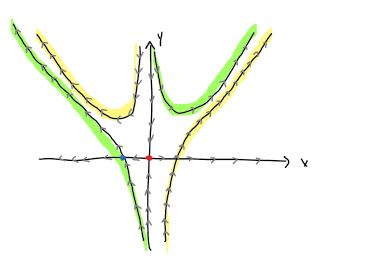
\includegraphics[width=0.8\textwidth]{phasenpotrait.jpeg}
    \end{center}

    %TODO: x-Achse falsch

    Die Informationen über die Richtung der Pfeile erhalten wir daher, dass der Eigenwert in $x$-Richtung $-1$ war, also in Richtung der $x$-Achse die Lösungen von Gleichgewichtspunkt weglaufen. In $y$-Richtung war der Eigenwert $-1$, d.h. Lösungen, die auf der $y$-Achse starten, werden zum Gleichgewichtspunkt hingezogen.
\end{enumerate}


\subsection{IV-13}

Wir bestimmen die Jacobi-Matrix der rechten Seite (die wir im Folgenden als $f$ bezeichnen):
\begin{equation*}
    J_f(x,y) = \qmatrix{-3 & 1 - 6y \\ -4 & 0} \then J_f(0,0) = \qmatrix{-3 & 1 \\ -4 & 0}
\end{equation*}
Diese hat die Sur $-3$ und die Determinante $4$.
Falls ihre Eigenwerte komplex sind, haben sie daher bei Realteil $- 1.5$ und falls sie reell sind, müssen sie dasselbe Vorzeichen haben und sich zu $- 3$ addieren, also auch beide negativ sein.
Somit ist der Gleichgewichtspunkt nach dem Prinzip der linearisierten Stabilität asymptotisch stabil.

Wir betrachten nun die Funktion
\begin{equation*}
    V(x,y) = 4x^2 - 2xy + y^2 + y^4\text{.}
\end{equation*}
Es handelt sich hierbei um eine Lyapunov-Funktion des Systems, denn
\begin{align*}
    \langle \nabla V(x,y), f(x,y) \rangle &= \left\langle \qmatrix{8x - 2y \\ -2x + 2y + 4y^3}, \qmatrix{-3x +y + 2y^3 \\ -4x}  \right\rangle\\
    &= -24x^2 + 8xy + 16xy^3 + 6xy - 2y^2 - 4y^4 + 8x^2 - 8xy - 16xy^3\\
    &= -16x^2 + 6xy - 2y^2 - 4y^4 = -7x^2 - y^2 - 4y^4 -(9x^2 - 6xy + y^2)\\
    &= =16x^2 - y^2 - 4y^4 - (3x - y)^2 \leq 0\text{,}
\end{align*}
wobei Gleichheit genau für $(x,y) = 0$ gilt. Es handelt sich also sogar um eine strikte Lyapunov-Funktion.
Es bleibt zu zeigen, dass $V(x,y)$ in $x,y$ ein lokales Minimum besitzt.
Hierzu bestimmen wir die Hesse-Matrix
\begin{align*}
    H_V(x,y) = \qmatrix{8 & -2 \\ -2 & 2 + 12y^2} \then H_V(0,0) = \qmatrix{8 & -2 \\ -2 & 2}
\end{align*}
und ihr charakteristisches Polynom
\begin{equation*}
    \chi_V(\lambda) = (8 - \lambda)(2 - \lambda) - 4 = \lambda^2 - 10 \lambda + 12
\end{equation*}
sowie dessen Nullstellen
\begin{equation*}
    \lambda_{1/2} = \frac{10 \pm \sqrt{100 - 48}}{2} = \frac{10 \pm \overbrace{\sqrt{52}}^{< 10}}{2} > 0\text{.}
\end{equation*}
Somit besitzt $V$ in $(0,0)$ ein (striktes) lokales Minimum und nach Lyapunov ist der Gleichgewichtspunkt $(0,0)$ somit asymptotisch stabil.

\subsection{IV-14}

\begin{enumerate}
    \item Für $\zeta = 1$ und $\zeta = -1$ ist die eindeutige maximale Lösung stationär und somit insbesondere nicht streng monoton fallend.
    
    Falls $\zeta \in (-1,1)$, so kann die Trajektorie der entsprechenden Lösung $\phi_\zeta$ die Trajektorien der beiden konstanten Lösungen nicht schneiden, also gilt $\phi_\zeta(t) \in (-1,1)$ für alle $t \in I_\zeta$. 
    Dann gilt $\phi_\zeta'(t) = f(\phi_\zeta(t)) > 0$, denn $f > 0$ auf $(-1, 1)$, da $f(0) > 0$ und aufgrund der Stetigkeit von $f$, des Zwischenwertsatz und der Absenz weiterer Nullstellen kein Vorzeichenwechsel stattfinden kann. 
    Also ist $\phi_\zeta$ streng monoton steigend.

    Falls $\zeta \in (-\infty, -1)$, kann $\phi_\zeta$ analog das Intervall $(-\infty, -1)$ nicht verlassen und da $f$ hier mit paralleler Argumentation ebenfalls positiv ist, muss $\phi_\zeta$ auch hier streng monoton steigend.

    Es verbleibt noch $\zeta \in (1, \infty)$. Analog zu den beiden oberen Fällen kann $\phi_\zeta$ das Intervall $(1, \infty)$ nicht verlassen und $f$ ist dort negativ, also ist $\phi_\zeta$ streng monoton fallend.

    Zusammenfassend ist $\phi_\zeta$ streng monoton fallend $\iff \zeta \in (1, \infty)$ und streng monoton steigend $\iff \zeta \in (-\infty, -1) \cup (-1, 1)$.
    \item Falls $\zeta = -1$ oder $\zeta = 1$ so ist $\phi_\zeta$ als konstante Lösung auf ganz $\mathds{R}$ existent.
    
    Sei nun $\zeta \in (-1,1)$.
    Wie bereits oben diskutiert kann dann $\phi_\zeta$ das Intervall $(-1, 1)$ und damit insbesondere das kompakte Intervall $[-1,1]$ nicht verlassen.
    Somit ist $\phi_\zeta$ auf $[0, t_\omega)$ (mit $t_\omega$ dem rechten Rand des maximalen Lösungsintervalls) beschränkt und nach Korollar 3.8 folgt damit $t_\omega = \infty$, also ist $\phi_\zeta$ auf $[0, \infty]$ existent. (Speziell für $\zeta \in (-1,1)$ lässt sich hier auch $I_\zeta = \mathds{R}$ zeigen).

    Für $\zeta \in (-\infty, -1)$ ist $\phi_\zeta(0) = \zeta$ und $\phi_\zeta(t) > \zeta$ für alle $t \in [0, t_\omega)$ ist streng monoton steigend.
    Da weiterhin $\phi_\zeta(t) < -1$ für all diese $t$ gelten muss, ist $\phi_\zeta$ also auf $[0, t_\omega)$  durch $[\zeta, -1]$ beschränkt somit gilt nach Korollar 3.8 $t_\omega = \infty$.

    Analog zeigt man, dass $\phi_\zeta$ für $\zeta \in (1, \infty)$ auf $[0, t_\omega)$ durch $[1, \zeta]$ beschränkt ist und auch hier $t_\omega = \infty$ gilt.

    \item Wir betrachten die Funktion
    \begin{equation*}
        V(x) = \frac{x^4}{4} + \frac{x^3}{3} - \frac{x^2}{2} - x 
    \end{equation*}
    mit Gradient
    \begin{equation*}
        \nabla V(x) = \frac{\partial}{\partial x} V(x) = x^3 + x^2 - x -1 = (x+1)^2(x-1) \text{.}
    \end{equation*}
    Dieser hat Nullstellen genau bei $-1, 1$ und die folgende Vorzeichenverteilung:
    \begin{align*}
        x \in (-\infty, -1) &\then \nabla V(x) < 0 \\
        x \in (-1, 1) &\then \nabla V(x) < 0 \\
        x \in (1, \infty) &\then \nabla V(x) > 0
    \end{align*}
    -- wie durch Betrachtung der Vielfachheit der Nullstellen sowie des Grenzverhaltens klar wird -- und somit gilt 
    \begin{align*}
        x \in (-\infty, -1) &\then \nabla V(x) \cdot f(x) < 0 \\
        x \in (-1, 1) &\then \nabla V(x) \cdot f(x) < 0 \\
        x \in (1, \infty) &\then \nabla V(x) \cdot f(x) < 0
    \end{align*}
    aufgrund der oben diskutierten Vorzeichenverteilung von $f$.
    Also gilt $\langle \nabla V(x), f(x)\rangle = \nabla V(x) \cdot f(x) \leq 0$ für alle $x \in \mathds{R}$ mit Gleichheit genau für $x = -1,1$. 
    Somit ist $V$ eine Lyapunov-Funktion von $f$ auf $\mathds{R}$.
    Auf $(0,2) \setminus \{1\}$ und $(-2, 0) \setminus \{-1\}$ ist $V$ sogar eine strikte Lyapunov-Funktion von $f$.

    Weiterhin hat $V$ bei $x_0 = 1$ eine (striktes) lokales (sogar globales) Minimum, denn die Ableitung $\nabla V$ hat dort eine Nullstelle und die zweite Ableitung $3x^2 + 2x - 1$ hat den Wert $4 > 0$.
    Somit ist $x_0 = 1$ nach dem Stabilitätskriterium von Lyapunov ein asymptotisch stabiler Gleichgewichtspunkt.

    Schließlich ist $x_0 = -1$ ein Terrassenpunkt von $V$, denn $V$ hat hier eine Nullstelle und die zweite Ableitung ebenfalls.
    Somit existiert in jeder Umgebung von $x_0 = -1$ ein $x$ mit $V(x) < V(x_0)$ und nach dem Instabilitätskriterium von Lyapunov ist $x_0 = -1$ somit ein instabiler Gleichgewichtspunkt von der DGL.
\end{enumerate}





\end{document}